\chapter{Methodology}
\label{ch:methodology}
\glsresetall

\section{Overview}

Initial experiments are completed to determine the optimal hyperparameters for the neural network. Networks are trained using multiple level of training noise to test for ideal performance. The optimal models will then be placed in a `Siamese network` --  a configuration that takes the classification values from multiple models and determines the `best fit` classification for the given input data.

\section{Targets}

  Five target models were chosen for this experiment. Each model is a missile-surrogate with a shared fuselage, and a unique nose cone. The dimensions of the fuselage and the nose cones are listed in table \ref{tab:models}. Nose cones 1-3 are simple cones with a fixed base diameter and edge length. Nose cones 4 and 5 are curved. They share the common 3 inch base diameter, with  differing diameters as they extend from the base to tip. The additional measurements represent the diameter of the cone at equally spaced intervals along the edge from base to tip. Each model is made of aluminum as is assumed to behave as a PEC in the presence of EMR. The Cad models of each missile nose is shown in figures \ref{nose_1_2}, \ref{nose_3_4}, and \ref{nose_5}. The side and top view of the missile is shown in figure \ref{fig:missile_body}.

  \begin{figure}[htbp]
    \centering
    \begin{subfigure}{.5\textwidth}
      \centering
      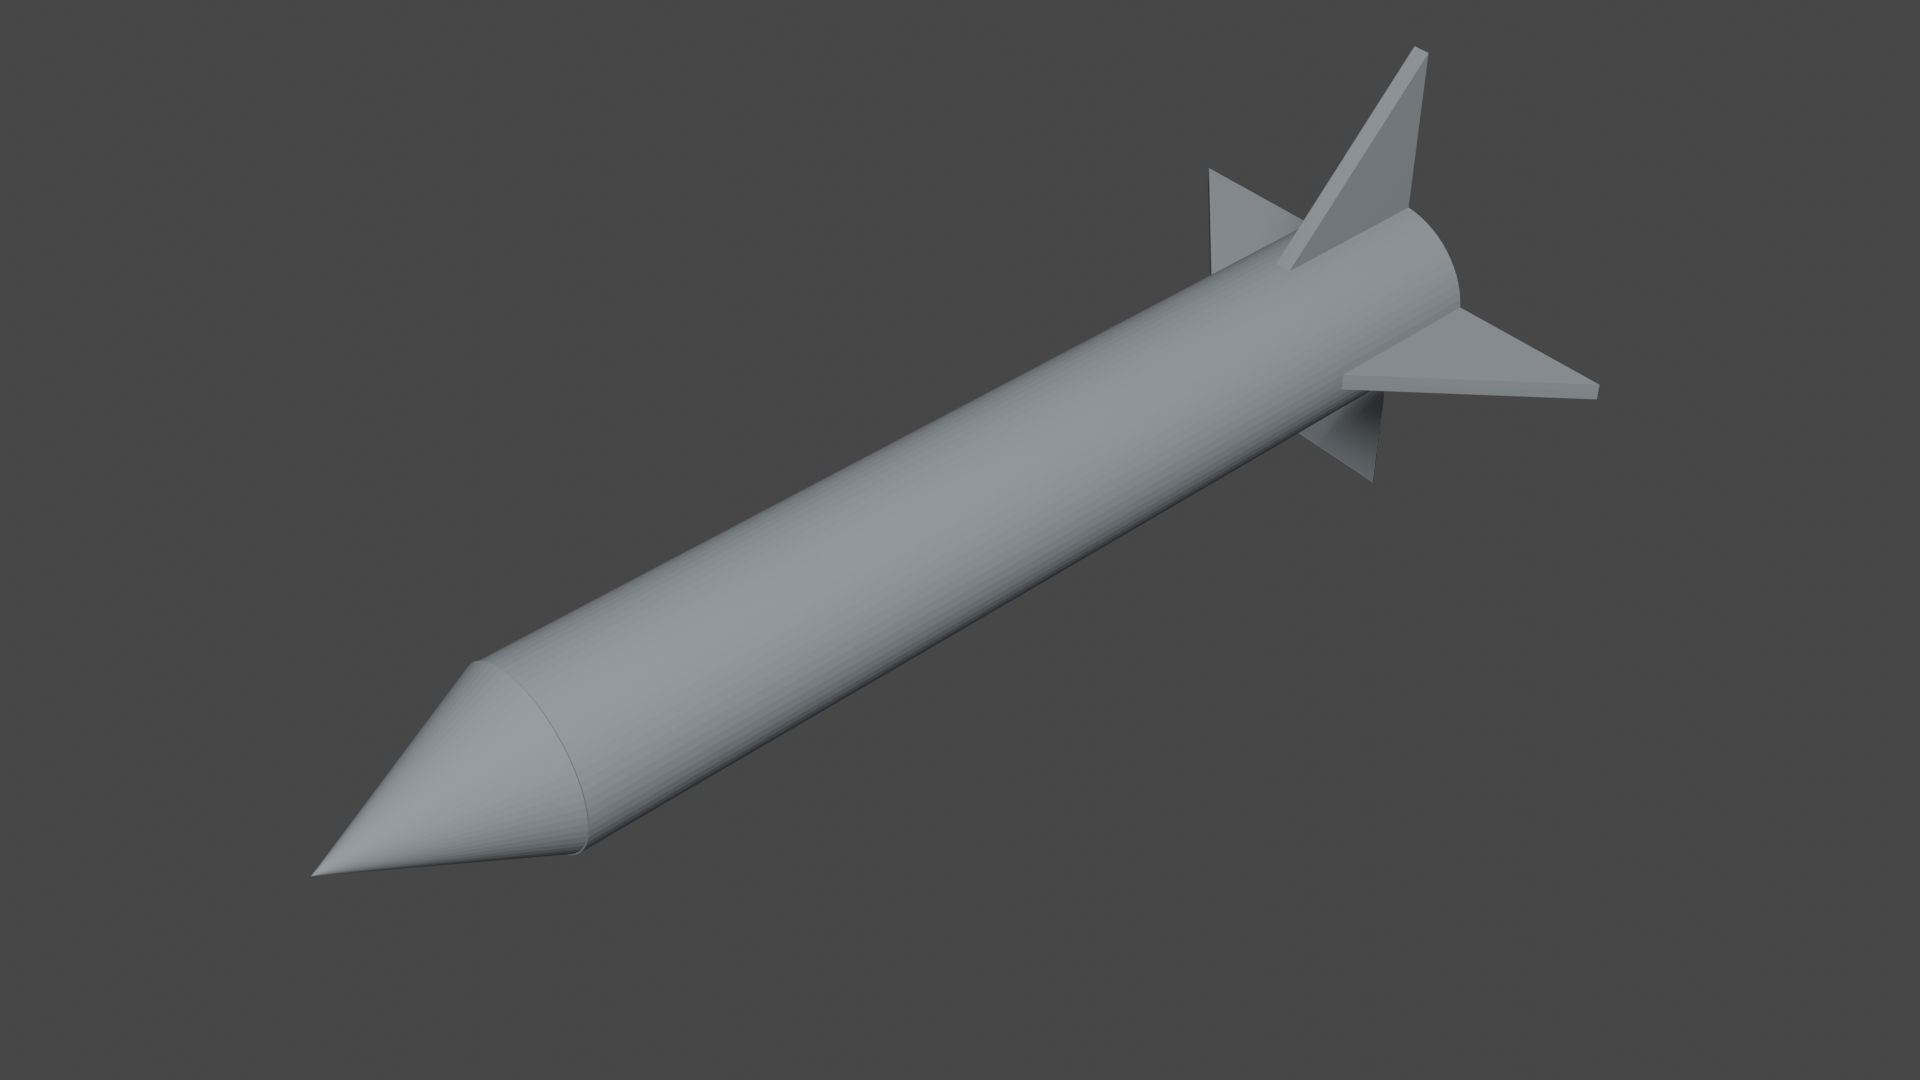
\includegraphics[width=.8\linewidth]{msl_side.png}
    \end{subfigure}%
    \begin{subfigure}{.5\textwidth}
      \centering
      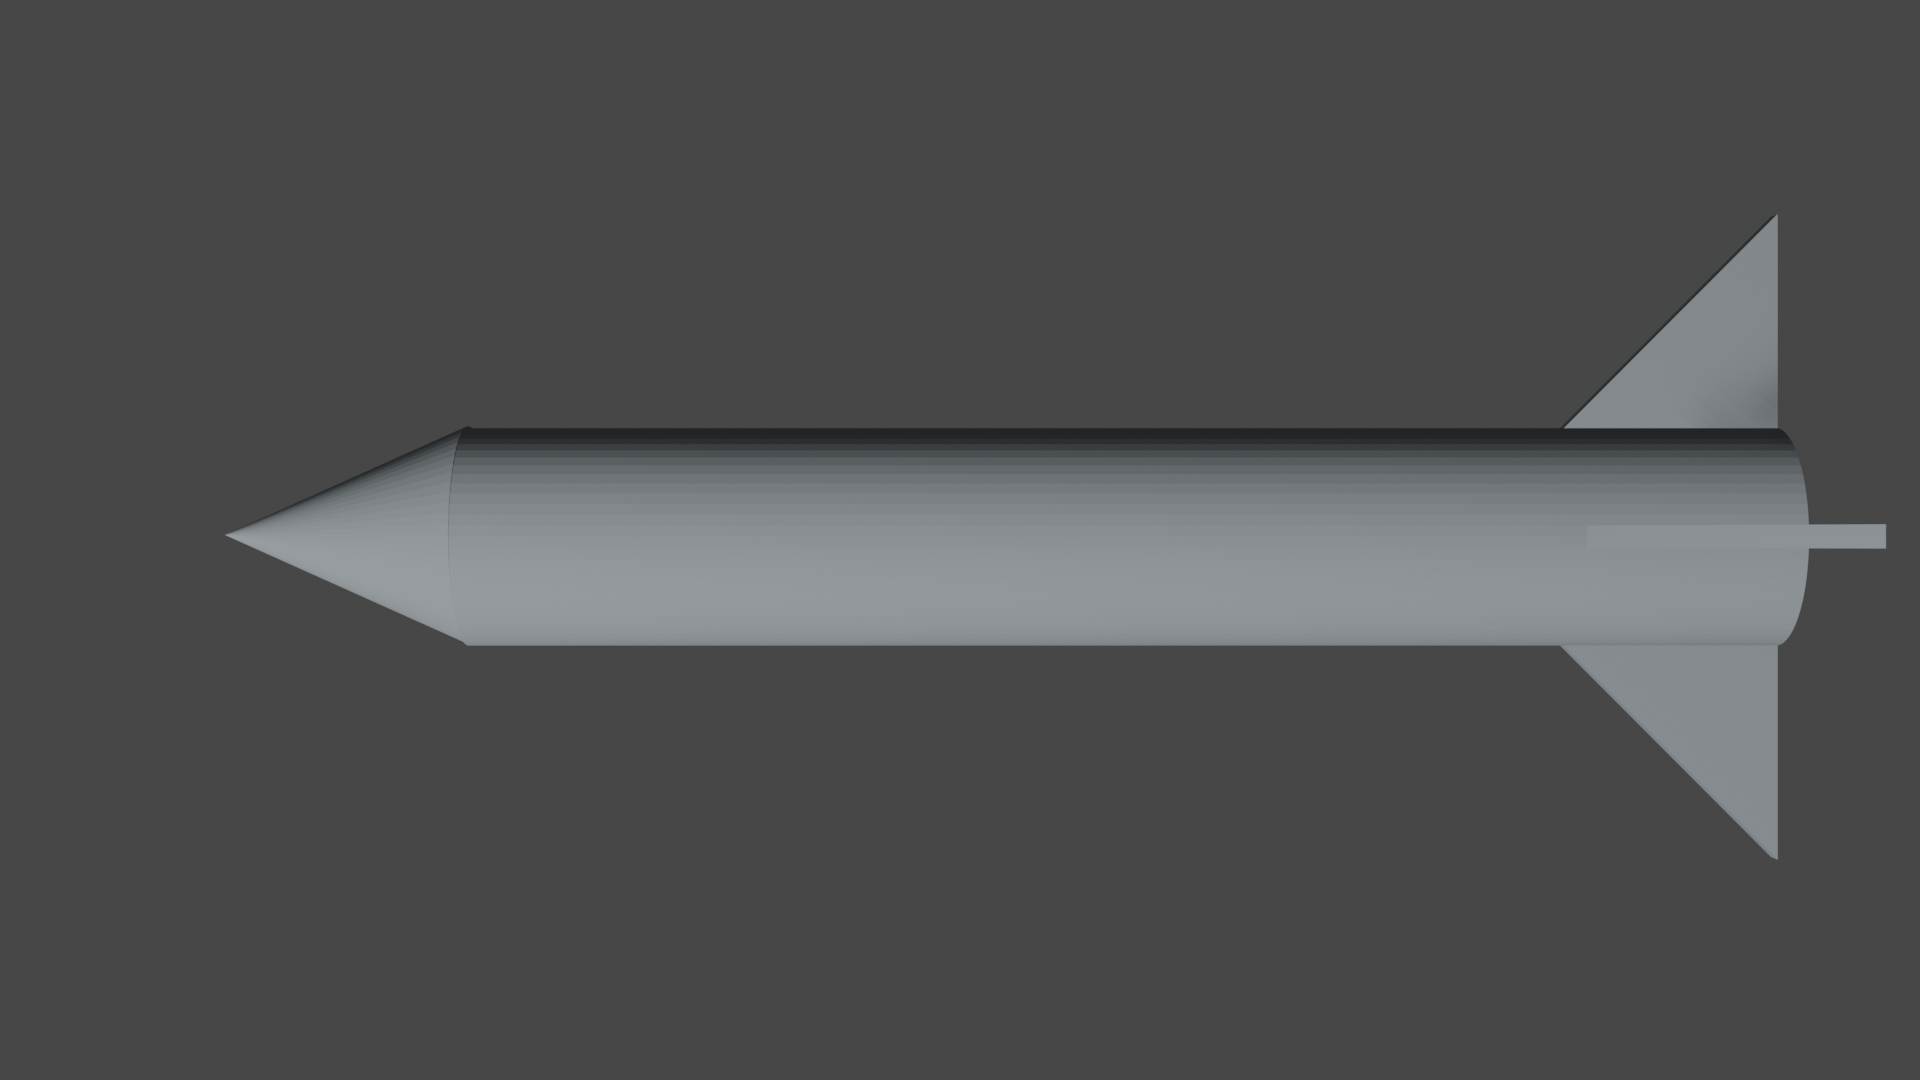
\includegraphics[width=.8\linewidth]{msl_top.png}
    \end{subfigure}
    \caption{Side and top view of the missile surrogate (Cad model)}
    \label{fig:missile_body}
  \end{figure}

  Simulation models were developed using Blender 3d, and exported as .stl mesh models. Mesh models were converted to solids form mesh, and exported as .step geometries using FreeCad. The .step format worked well with CADFeko's internal meshing system. Since Blender 3D does not export .step natively, the additional step of importing the .stl mesh into FreeCad was necessary.

\section{Measurement}
  The targets were measured at the Air Force Institute of Technologies (AFIT) Compact Radar Range. The layout of the AFIT range is shown in figure \ref{fig:range}. The range uses a BlueMax G6 instrumentation radar (blue items in schematic), with a Vivaldi wide-band antenna configured in both horizontal and vertical polarizations. Transmitted signals are directed at a curved reflector located 3 meters from the antenna. Ideally, the incident field will be a plane wave. That is, the wave front is the same when measured vertically or horizontally. However, the short distance between the antenna and the target will produce a curved wave-front surface. The reflector helps to `flatten' the wave front, and make it appear more planer.

  Targets are placed on a foam column located 7 meters from the reflector. The column is 2 meters tall, and can rotate 360 degrees. Foam is used, as its intrinsic properties are similar to air, and do not contribute significantly to scene clutter.

  \begin{figure}[htbp]
    \centering
    \begin{subfigure}{.8\textwidth}
      \centering
      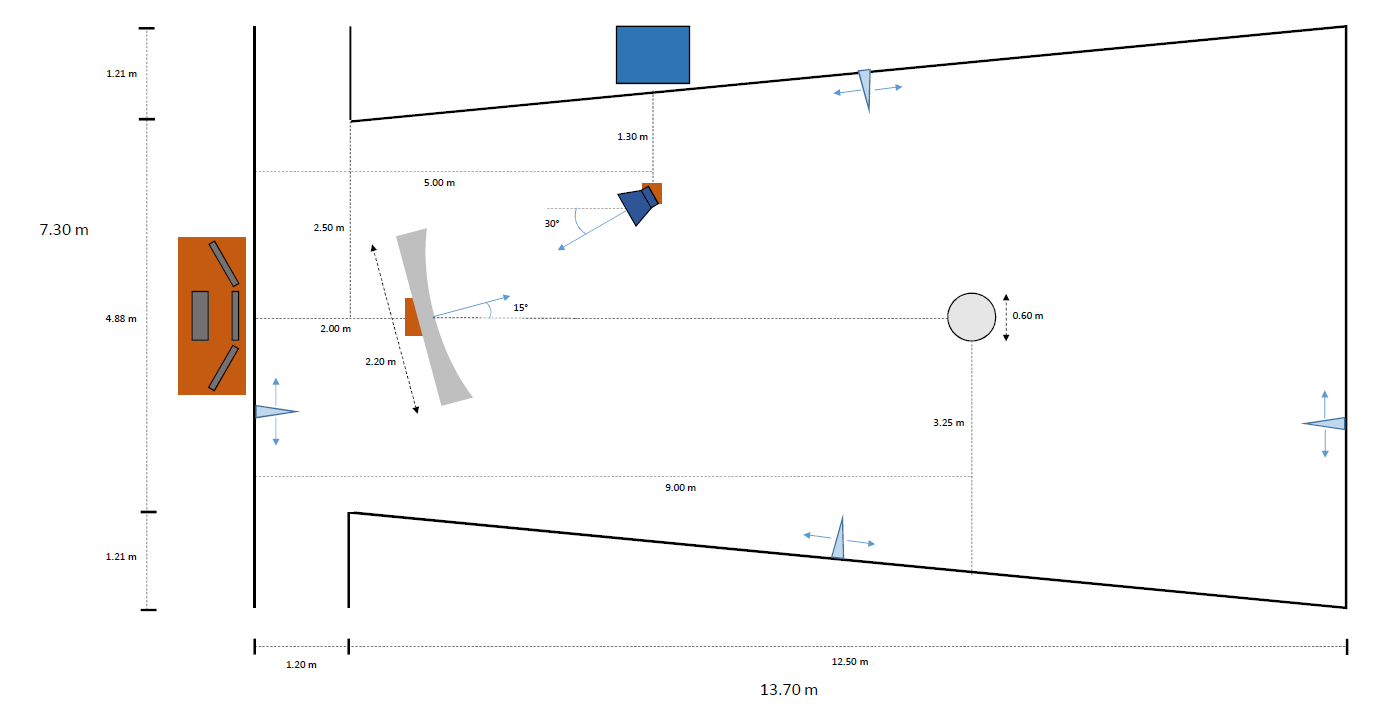
\includegraphics[width=.8\linewidth]{range.png}
    \end{subfigure}%
    \begin{subfigure}{.8\textwidth}
      \centering
      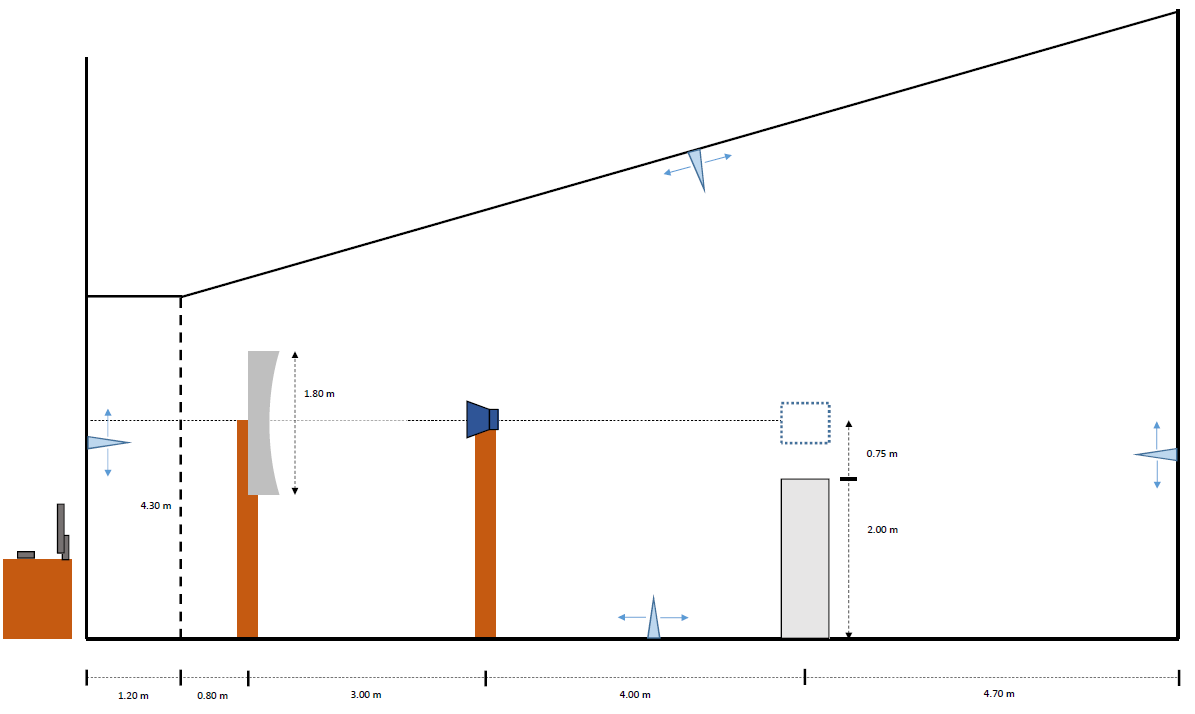
\includegraphics[width=.8\linewidth]{range_side.png}
    \end{subfigure}
    \caption[AFIT Compact Range Schematic]{Top-down and side view of the AFIT compact radar range.}
    \label{fig:range}
  \end{figure}

  The radar can capture measurements over multiple frequencies, polarizations, and target aspect-angles. Measurements are returned as complex voltages $M$. A measurement is collected using a specific carrier frequency $f$, at a single aspect angle $a$. For example, measurement $M_0$ is collected by launching a stream of pulses with carrier frequency $f_0$ at a target presenting a fixed aspect angle $a_0$. The receiver will collect and integrate $N$ echo pulses and store the value as $M(f_0, a_0)$. This process is repeated over the desired range of frequencies and angles resulting in a matrix

  \begin{equation}\label{eq:RCS_mat}
    E_{tt} =
     \begin{bmatrix}
       M_{0,0} & M_{0,1} & \cdots & M_{0,A} \\
       M_{1,0} & M_{1,1} & \cdots & M_{1,A} \\
       \vdots  & \vdots  & \ddots & \vdots  \\
       M_{F,0} & M_{F,1} & \cdots & M_{F,A}
     \end{bmatrix}
     \\
     E_{pp} =
      \begin{bmatrix}
      M_{0,0} & M_{0,1} & \cdots & M_{0,A} \\
      M_{1,0} & M_{1,1} & \cdots & M_{1,A} \\
      \vdots  & \vdots  & \ddots & \vdots  \\
      M_{F,0} & M_{F,1} & \cdots & M_{F,A}
      \end{bmatrix}
  \end{equation}

  where $E_{tt}$ and $E_{pp}$ represent measurements taken for the vertical and horizontally aligned incident wave polarization. Each row in the matrices corresponds to 360 aspect angles measured at one frequency. The total array shape is $F \times A$, where $F$ and $A$ are the number of frequencies and angles captured respectively.

  Table \ref{tab:m_params} lists the measurement parameters used for this experiment.

  \begin{table}
    \centering
    \begin{tabular}{|l|r|}
      \hline
      Transmitter Power: & $40$[dBm]\\
      \hline
      Tx Gain: $15$[dB]\\
      \hline
      Rx Gain: $15$[dB]\\
      \hline
      IF BW: $200$[kHz]\\
      \hline
      Noise Figure, $F$:  $3$[dB]\\
      \hline
      Tx Loss: $4.5$[dB]\\
      \hline
      Rx Loss: $4.5$[dB]\\
      \hline
      Operating Temp: $68$[F]\\
      \hline
      Pulse Width: & $10[ns]$\\
      \hline
      Frequency Range: & $4.5-5.5 [GHz]$, $10 [MHz]$ step\\
      \hline
      Aspect-angle Range: & $0-360 ^{\circ}$, $1^{\circ}$ step\\
      \hline
      Integration Factor: & $1024$ \\
      \hline
      Transmit Delay : & $330$ [ns] \\
      \hline
      Receiver Delay : & $434-446$ [ns] \\
      \hline
    \end{tabular}
    \caption{Measurement parameters.}
    \label{tab:m_params}
  \end{table}

  % TODO: add quiet zone information

  The radar used for this project produces a discrete RCS measurement at individual frequencies as opposed to a time domain response for each pulse. Since this time-domain information was unavailable, this experiment attempts to recreate the time-domain response, by capturing discrete measurements for each frequency and stitching them together into a frequency domain equivalent for the expected time-domain response.

  The integration factor was chosen to provide sufficiently accurate measurements. This ideal measurement serves as a signal to noise performance baseline. The receiver delay of $434-446$ [ns] puts the quiet zone window at approximately 76 meters when accounting for the reducing transmission speed of waves in transmission line. The target fixture is located 14 meters from the antenna, with the remaining distance accounted for by feedline from the instrument to the antenna. This window was confirmed by `walking` the range. This operation transmits pulses from the antenna, and shifts the reception window until a known target is captured in the desired quiet zone.

\section{Simulation}

  Simulations were completed using Altair's CADFeko Electromagnetic Simulation Suite. CADFeko uses an iterative \gls{MOM-SEP} algorithm to compute the RCS response of the target model. The output data from the simulation is in phasor form. Method of Moments is used to calculate scattering for targets in the resonant regime:  when physical target size is roughly the same size as the incident wave length, but less than 10 times larger \cite{Knott}. At 5 GHz, the incident wave length is 60 millimeters. At 457mm, the fuselage body is 7.62 times larger than the 5 GHz wavelength placing towards the upper end of the resonant regime. The nose cones range in size from 101 to 228 mm, which fit comfortably in the resonant regime.

\section{Data Processing}

  \subsection{Data Set Generation}
    In order to mimic the expected response of a radar pulse, training and test data sets are built by slicing the RCS matrices shown in equation \ref{eq:RCS_mat} column wise. The resulting vectors

    \begin{equation}\label{eq:F_vec}
      F_{tt}(f, a_n) =
       \begin{bmatrix}
         M_{0, a_n} & M_{1,a_n} & \cdots & M_{F,a_n}
       \end{bmatrix},\,\,
       \\
     F_{pp}(f, a_n) =
      \begin{bmatrix}
        M_{0, a_n} & M_{1,a_n} & \cdots & M_{F,a_n}
      \end{bmatrix}
      \\
    \end{equation}

    contain the measurements $M(f, a_n)$ for all frequencies $f$, at a specified angle $a_n$ for the vertical and horizontal polarizations respectively. Each vector corresponds to the frequency content of an integrated pulse stream for each pose angle of the target. The training data set can be made arbitrarily large by multiplying frequency slices and applying random additive noise with power $N_{train}$ to create variance in each sample.

    Each sample in the training data set is assigned a label that corresponds to the `sector' that each sample falls in. Sectors are chosen such that RCS characteristics specific to the target fall in the same sector. This experiment utilizes either 3 or 4 90-degree sectors centered on the nose, tail, and sides of the target. The three label case collapses the sides of the fuselage into a single label.

    Test data sets are built similarly:  frequency vectors  are extracted from the measurement array, and additive noise with power level $N_{test}$ is applied.

  \subsection{Data Augmentation}
  \label{sec:DA}

    During training, neural networks optimize their decision weights by utilizing an `optimizer'. An optimizer is a method of testing whether the network is adjusting it weights in a way that maximizes its ability to categorize the input data correctly. This experiment utilizes a Stochastic Gradient Descent optimizer (SGD). This method favors adjustments in the networks weights that push towards a minimization of error in categorization. Since this is a method that utilizes slopes, differentiation is employed. In order to prevent unnecessarily large slopes, data is augmented. There are two forms of data augmentation that are typically employed: standardization, and normalization.

    Standardization takes the maximum value in the current training array, and scales the entire array. This creates a data range between 0 and 1. Standardization of data in this experiment is done using

    \begin{equation}\label{eq:F_stan}
      F_{tt}(f, a_n) =
       \begin{bmatrix}
         M_{0, a_n} & M_{1,a_n} & \cdots & M_{F,a_n}
       \end{bmatrix} / max(F_{tt}(f, a_n))
    \end{equation}

    where the function $max()$ pulls the max value in the vector.

    Normalization extracts the mean and standard deviation of the vector and returns a `Z-Score' for the each cell in the array using

    \begin{equation}\label{eq:F_z}
      F_{tt}(f, a_n) =
       \frac{\left(
       \begin{bmatrix}
         M_{0, a_n} & M_{1,a_n} & \cdots & M_{F,a_n}
       \end{bmatrix}
        - \mu \right)}{\sigma}
    \end{equation}

    where $\mu$ is the mean value of the vector, and $\sigma$ is the standard deviation.

  \subsection{Comparison}
  \label{sec:comparison}

    Signals are compared using a cross-correlation function. The cross correlation function measures the similarity between two signals, and outputs a correlation coefficient, $\rho$. Values for $\rho$ range from $\pm 1$ for correlated, and anti-correlated signals respectively, and $0$ for un-correlated signals. As an example, the cross correlation of a signal with itself, will have $\rho=1$.

    Signal similarity is measured over all frequencies, at each angle using

    \begin{equation}\label{eq:corr}
      \rho = Corr( E_{1, tt/pp}(f, a_i), E_{2, tt/pp}(f, a_i)  )
    \end{equation}

    where $E_{1, pol}$ and $E_{2, pol}$ RCS phasor response measurements for signals 1 and 2, at angle $a_i$ and polarization $pol$, over all frequencies $f$. Signals will be selected from the pool of simulated and measured RCS response. Measuring the correlation strength of all targets with one another will serve as a means of identifying breakdowns in target classification. The correlation function is always applied to signals with similar polarizations.

    To measure the breakdown in signal correlation as noise is applied, the following algorithm is employed:

    \begin{enumerate}
      \item Signals 1 and 2 are selected
      \item Noise is applied to signal 1 and signal 2
      \item Signals one and two are augmented per angle
      \item Equation \ref{eq:corr} is applied for each angle
      \item The resulting vector of correlation coefficients is plotted against angle
    \end{enumerate}

    Correlation performance is reported in SNR. The SNR for each target is the average phasor value of all data elements in the matrices $E_{tt}$ and $E_{pp}$ for each target.


\section{Neural Network Development}




\section{RCS Calculation}
